\chapter{Wireless Architectures}\label{wireless-architectures}

802.11 MESSAGE / FRAME FORMAT

\begin{figure}
\centering
\pandocbounded{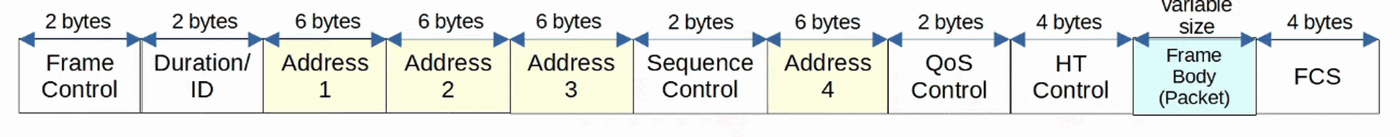
\includegraphics[keepaspectratio,alt={image}]{images/59-wireless-architecutres/img-001.png}}
\end{figure}

\begin{itemize}
\tightlist
\item
  802.11 FRAMES have a different format than 802.3 ETHERNET FRAMES
\item
  For the CCNA, you don't have to learn it in as much detail as the
  ETHERNET and IP HEADERS
\item
  Depending on the 802.11 VERSION and the MESSAGE TYPE, some of the
  fields might not be present in the FRAME

  \begin{itemize}
  \tightlist
  \item
    For example: Not ALL messages use all 4 ADDRESS FIELDS
  \end{itemize}
\item
  FRAME CONTROL

  \begin{itemize}
  \tightlist
  \item
    Provides information such as MESSAGE TYPE and SUBTYPE
  \item
    Indicates if the FRAME is a MANAGEMENT frame
  \end{itemize}
\item
  DURATION / ID

  \begin{itemize}
  \tightlist
  \item
    Depending on the MESSAGE TYPE, this field can indicate:

    \begin{itemize}
    \tightlist
    \item
      The TIME (in microseconds) the CHANNEL will be dedicated to
      transmission of the FRAME
    \item
      Identifier for the ASSOCIATION (the connection)
    \end{itemize}
  \end{itemize}
\item
  ADDRESSES

  \begin{itemize}
  \tightlist
  \item
    Up to FOUR ADDRESSES can be present in an 802.11 FRAME.
  \item
    Which ADDRESSES are present, and their ORDER, depends on the MESSAGE
    TYPE

    \begin{itemize}
    \tightlist
    \item
      DESTINATION ADDRESS (DA) : Final RECIPIENT of the FRAME
    \item
      SOURCE ADDRESS (SA) : Original SENDER of the FRAME
    \item
      RECEIVER ADDRESS (RA) : Immediate RECIPIENT of the FRAME
    \item
      TRANSMITTER ADDRESS (TA) : Immediate SENDER of the FRAME
    \end{itemize}
  \end{itemize}
\item
  SEQUENCE CONTROL

  \begin{itemize}
  \tightlist
  \item
    Used to reassemble FRAGMENTS and eliminate DUPLICATE FRAMES
  \end{itemize}
\item
  QoS CONTROL

  \begin{itemize}
  \tightlist
  \item
    Used in QoS to PRIORITIZE certain traffic
  \end{itemize}
\item
  HT (High Throughput) CONTROL

  \begin{itemize}
  \tightlist
  \item
    Added in 802.11n to ENABLE High Throughput operations
  \item
    802.11n is also known as ``HIGH THROUGHPUT'' (HT) WI-FI
  \item
    802.11ac is also know as ``VERY HIGH THROUGHPUT'' (VHT) WI-FI
  \end{itemize}
\item
  FCS (FRAME CHECK SEQUENCE)

  \begin{itemize}
  \tightlist
  \item
    Same as in an ETHERNET FRAME, used to check for errors
  \end{itemize}
\end{itemize}

802.11 ASSOCIATION PROCESS

\begin{itemize}
\tightlist
\item
  ACCESS POINTS bridge traffic between WIRELESS STATIONS and other
  DEVICES
\item
  For a STATION to send traffic through the AP, it must be associated
  with the AP
\item
  There are THREE 802.11 CONNECTION STATES:

  \begin{itemize}
  \tightlist
  \item
    NOT AUTHENTICATED, NOT ASSOCIATED
  \item
    AUTHENTICATED, NOT ASSOCIATED
  \item
    AUTHENTICATED and ASSOCIATED
  \end{itemize}
\item
  The STATION must be AUTHENTICATED and ASSOCIATED with the AP to send
  traffic through it
\end{itemize}

\begin{figure}
\centering
\pandocbounded{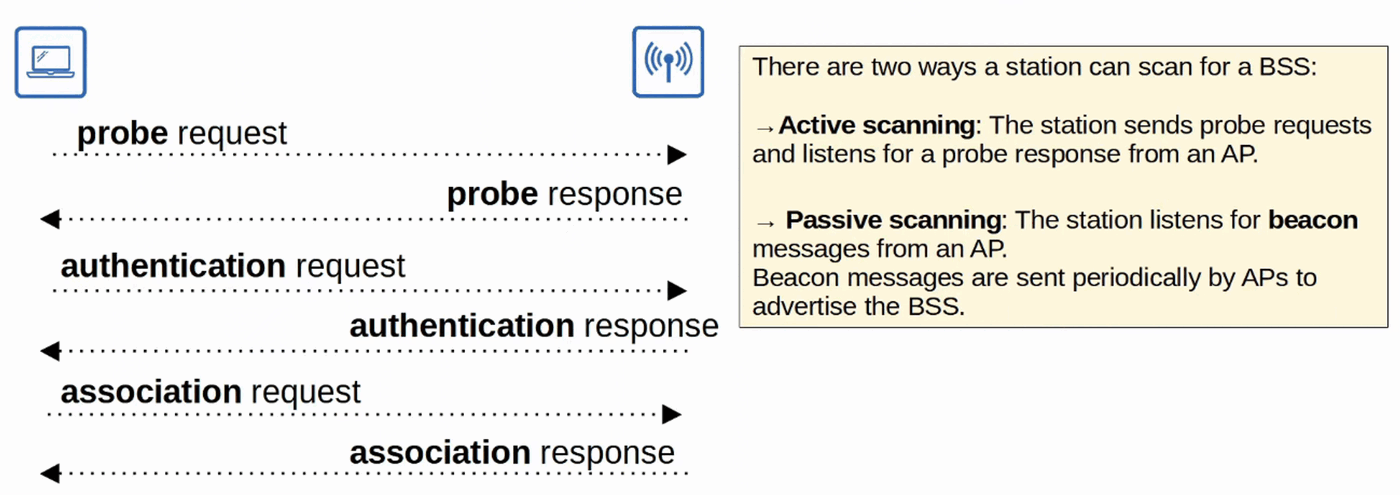
\includegraphics[keepaspectratio,alt={image}]{images/59-wireless-architecutres/img-002.png}}
\end{figure}

802.11 MESSAGE TYPES

\begin{itemize}
\tightlist
\item
  There are THREE 802.11 MESSAGE TYPES

  \begin{itemize}
  \tightlist
  \item
    MANAGEMENT
  \item
    CONTROL
  \item
    DATA
  \end{itemize}
\item
  MANAGEMENT

  \begin{itemize}
  \tightlist
  \item
    Used to manage the BSS

    \begin{itemize}
    \tightlist
    \item
      BEACON
    \item
      PROBE REQUEST / PROBE RESPONSE
    \item
      AUTHENTICATION
    \item
      ASSOCIATION REQUEST / ASSOCIATION RESPONSE
    \end{itemize}
  \end{itemize}
\item
  CONTROL

  \begin{itemize}
  \tightlist
  \item
    Used to control access to the medium (RADIO FREQUENCY)
  \item
    Assists with delivery of MANAGEMENT and DATA FRAMES

    \begin{itemize}
    \tightlist
    \item
      RTS (REQUEST TO SEND)
    \item
      CTS (CLEAR TO SEND)
    \item
      ACK
    \end{itemize}
  \end{itemize}
\item
  DATA

  \begin{itemize}
  \tightlist
  \item
    Used to send actual DATA PACKETS
  \end{itemize}
\end{itemize}

AUTONOMOUS APs

\begin{itemize}
\tightlist
\item
  AUTONOMOUS APs are self-contained SYSTEMS that do NOT RELY on a WLC
\item
  AUTONOMOUS APs are configured individually

  \begin{itemize}
  \tightlist
  \item
    Can be configured by CONSOLE cable (CLI)
  \item
    Can be configured by TELNET (CLI)
  \item
    Can be configured by HTTP / HTTPS Web connection (GUI)
  \item
    An IP ADDRESS for REMOTE MANAGEMENT should be configured
  \item
    The RF PARAMETERS must be manually configured (Transmit Power,
    Channel, etc)
  \item
    SECURITY POLICIES are handled individually by each AP
  \item
    QoS RULES etc. are configured individually by each AP
  \end{itemize}
\item
  There is NO CENTRAL MONITORING or MANAGEMENT of APs
\end{itemize}

\begin{figure}
\centering
\pandocbounded{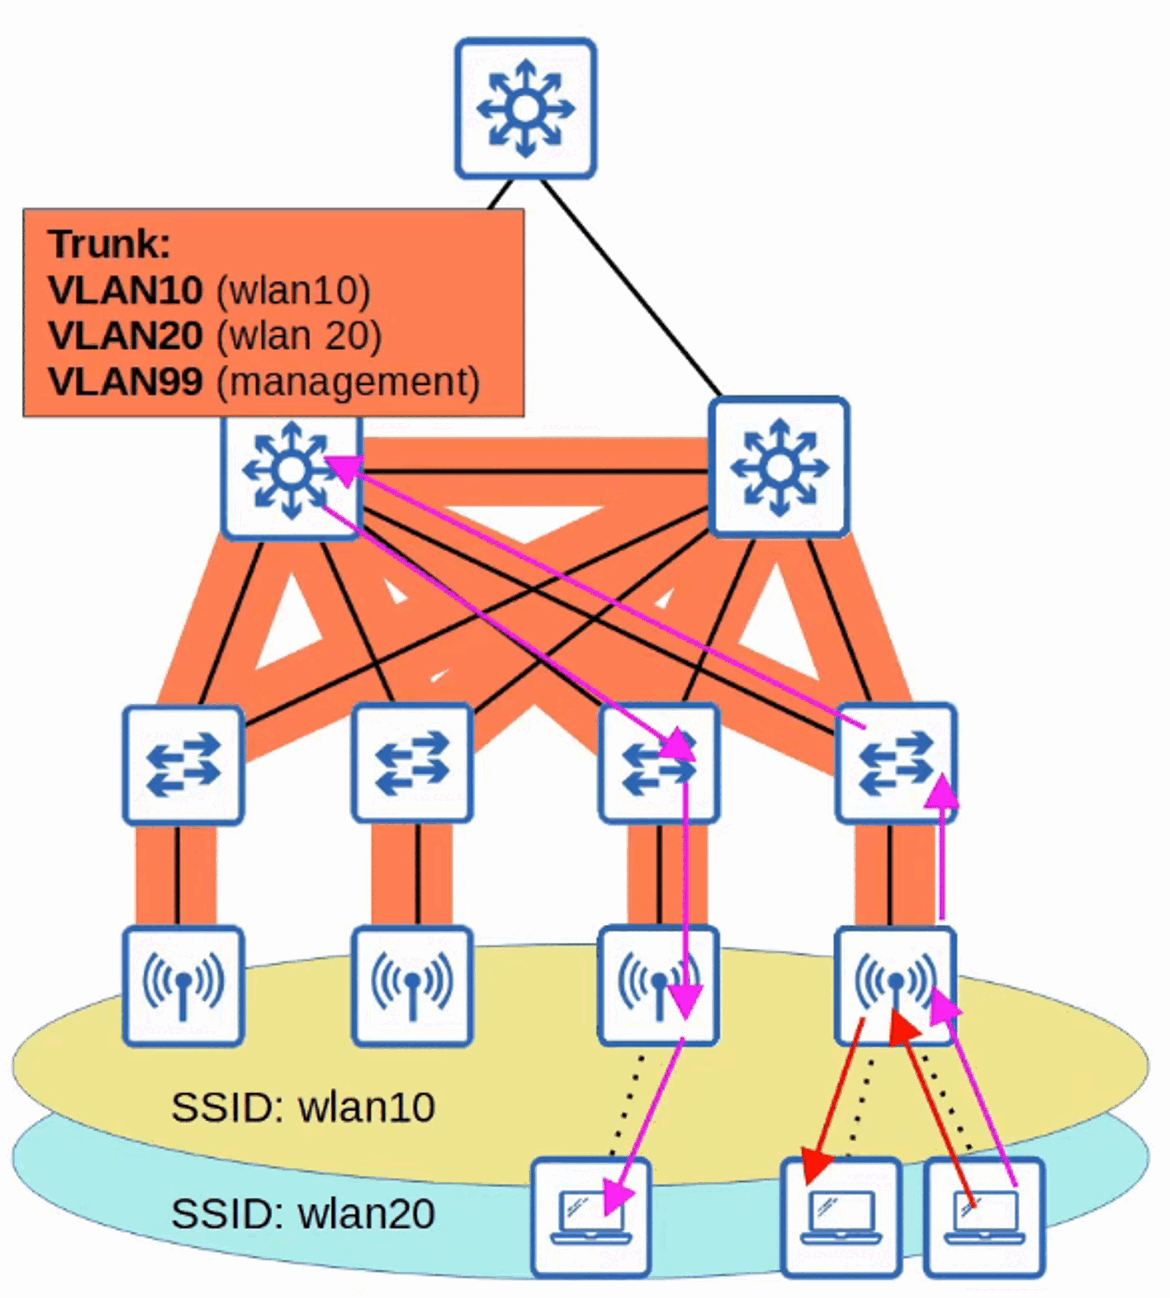
\includegraphics[keepaspectratio,alt={image}]{images/59-wireless-architecutres/img-003.png}}
\end{figure}

\begin{itemize}
\tightlist
\item
  AUTONOMOUS APs connect to the WIRED NETWORK with a TRUNK link
\item
  DATA traffic from WIRELESS CLIENTS have a very direct PATH to the
  WIRED NETWORK or to other WIRELESS CLIENTS associated with the same AP
\item
  Each VLAN has to STRETCH across the entire NETWORK. This is considered
  BAD practice

  \begin{itemize}
  \tightlist
  \item
    Large Broadcast Domains
  \item
    Spanning Tree will disable links
  \item
    Adding / Deleting VLANs is VERY labor-intensive
  \end{itemize}
\item
  AUTONOMOUS APs can be used in SMALL NETWORKS but they are not viable
  in MEDIUM to LARGE NETWORKS

  \begin{itemize}
  \tightlist
  \item
    LARGE NETWORKS can have thousands of APs
  \end{itemize}
\item
  AUTONOMOUS APs can also function in the modes covered in the previous
  video:

  \begin{itemize}
  \tightlist
  \item
    REPEATER
  \item
    OUTDOOR BRIDGE
  \item
    WORKGROUP BRIDGE
  \end{itemize}
\end{itemize}

LIGHTWEIGHT APs

\begin{itemize}
\item
  The functions of an AP can be split between the AP and a WIRELESS LAN
  CONTROLLER (WLC)
\item
  The is what is called SPLIT-MAC ARCHITECTURE
\item
  LIGHTWEIGHT APs handle \textbf{``real-time''} operations like:

  \begin{itemize}
  \tightlist
  \item
    TRANSMITTING / RECEIVING RF TRAFFIC
  \item
    ENCRYPTION / DECRYPTION OF TRAFFIC
  \item
    SENDING OUT BEACONS / PROBES
  \item
    PACKET PRIORITIZATION
  \item
    Etc\ldots{}
  \end{itemize}
\item
  WLC Functions (not time dependent)

  \begin{itemize}
  \tightlist
  \item
    RF MANAGEMENT
  \item
    SECURITY / QoS MANAGEMENT
  \item
    CLIENT AUTHENTICATION
  \item
    CLIENT ASSOCIATION / ROAMING MANAGEMENT
  \item
    RESOURCE ALLOCATION
  \item
    Etc\ldots{}
  \end{itemize}
\item
  The WLC is also used to centrally configured the lightweight APs
\item
  The WLC can be located in the same SUBNET / VLAN as the lightweight
  APs it manages OR in a different SUBNET / VLAN
\item
  The WLC and the lightweight APs AUTHENTICATE each other using DIGITAL
  CERTIFICATES installed on each DEVICE ( X.509 STANDARD CERTIFICATES )

  \begin{itemize}
  \tightlist
  \item
    This ensures that only AUTHORIZED APs can join the NETWORK
  \end{itemize}
\end{itemize}

\begin{figure}
\centering
\pandocbounded{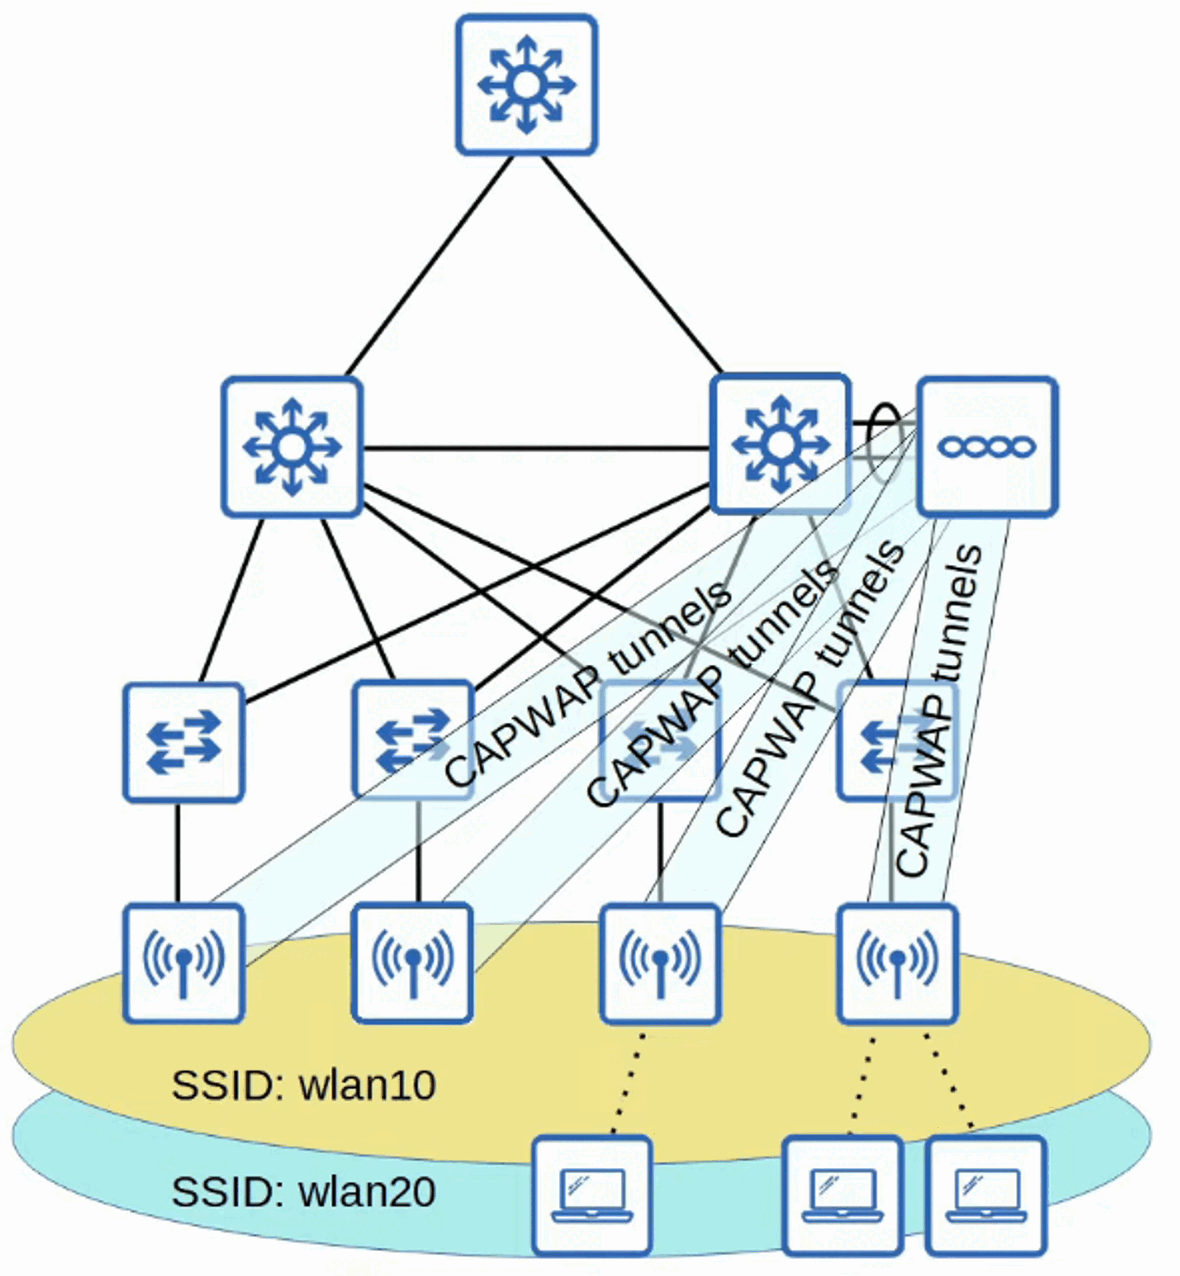
\includegraphics[keepaspectratio,alt={image}]{images/59-wireless-architecutres/img-004.png}}
\end{figure}

\begin{itemize}
\item
  THE WLC and lightweight APs use a PROTOCOL called CAPWAP (CONTROL AND
  PROVISIONING OF WIRELESS ACCESS POINTS) to communicate

  \begin{itemize}
  \tightlist
  \item
    Based on an older PROTOCOL called LWAPP (LIGHTWEIGHT ACCESS POINT
    PROTOCOL)
  \end{itemize}
\item
  TWO TUNNELS are created between each AP and the WLC :

  \begin{itemize}
  \tightlist
  \item
    CONTROL TUNNEL (UDP Port 5246)

    \begin{itemize}
    \tightlist
    \item
      This TUNNEL is used to configure the APs and control and manage
      operations
    \item
      All traffic in this TUNNEL is ENCRYPTED, by default
    \end{itemize}
  \item
    DATA TUNNEL (UDP Port 5247)

    \begin{itemize}
    \tightlist
    \item
      All traffic from WIRELESS CLIENTS is sent through this TUNNEL to
      the WLC
    \item
      IT DOES NOT GO DIRECTLY TO THE WIRED NETWORK !
    \end{itemize}
  \end{itemize}
\item
  Traffic in this TUNNEL is not ENCRYPTED by default but you can
  configure it to be ENCRYPTED with DTLS (DATAGRAM TRANSPORT LAYER
  SECURITY)
\item
  Because ALL traffic from WIRELSS CLIENTS is TUNNELED to the WLC with
  CAPWAP, APs connect to the SWITCH ACCESS PORTS - NOT TRUNK PORTS
\end{itemize}

\begin{figure}
\centering
\pandocbounded{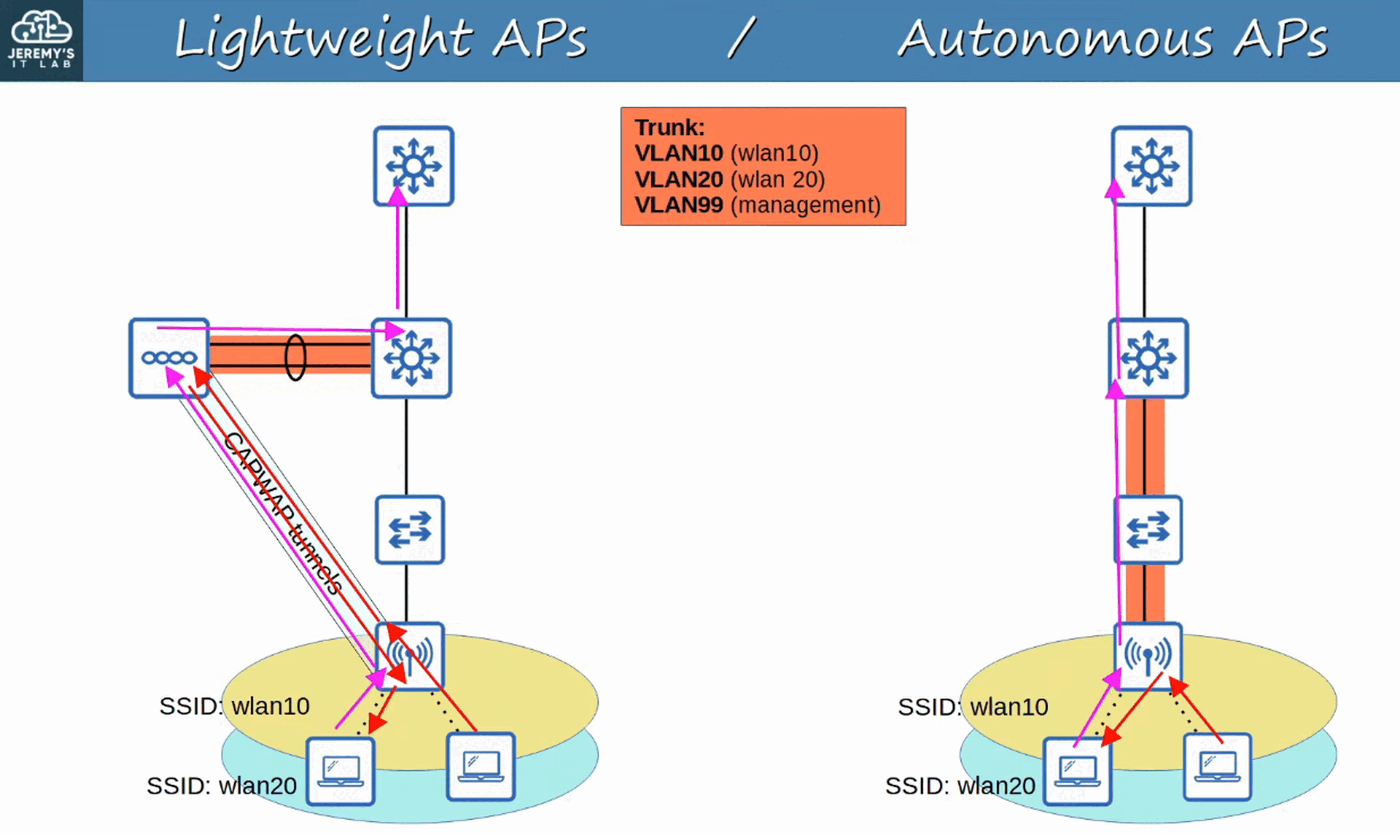
\includegraphics[keepaspectratio,alt={image}]{images/59-wireless-architecutres/img-005.png}}
\end{figure}

*** (Not necessary to MEMORIZE for CCNA) ***

There are some KEY BENEFITS to SPLIT-MAC ARCHITECTURE

\begin{itemize}
\tightlist
\item
  SCALABILITY

  \begin{itemize}
  \tightlist
  \item
    With a WLC (or multiple) it's SIMPLER to build and support a NETWORK
    with thousands of APs
  \end{itemize}
\item
  DYNAMIC CHANNEL ASSIGNMENT

  \begin{itemize}
  \tightlist
  \item
    The WLC can automatically select which channel each AP should use
  \end{itemize}
\item
  TRANSMIT POWER OPTIMIZATION

  \begin{itemize}
  \tightlist
  \item
    The WLC can automatically set the appropriate transmit power for
    each AP
  \end{itemize}
\item
  SELF-HEALING WIRELESS COVERAGE

  \begin{itemize}
  \tightlist
  \item
    When an AP stops functioning, the WLC can increase the transmit
    power of nearby APs to avoid coverage holes
  \end{itemize}
\item
  SEAMLESS ROAMING

  \begin{itemize}
  \tightlist
  \item
    CLIENTS can roam between APs with no noticeable delay
  \end{itemize}
\item
  CLIENT LOAD BALANCING

  \begin{itemize}
  \tightlist
  \item
    If a CLIENT is in range of TWO APs, the WLC can associate the CLIENT
    with the least-used AP, to balance the load among APs
  \end{itemize}
\item
  SECURITY / QoS MANAGEMENT

  \begin{itemize}
  \tightlist
  \item
    Central management of SECURITY and QoS policies ensures consistency
    across the NETWORK
  \end{itemize}
\item
  LIGHTWEIGHT APs can be configured to operate in VARIOUS MODES:

  \begin{itemize}
  \tightlist
  \item
    LOCAL

    \begin{itemize}
    \tightlist
    \item
      This is the DEFAULT mode where the AP offers a BSS (more multiple
      BSSs) for CLIENTS to associate with
    \end{itemize}
  \item
    FLEXCONNECT

    \begin{itemize}
    \tightlist
    \item
      Like a LIGHTWEIGHT AP in LOCAL mode, it offers ONE or MORE BSSs
      for CLIENTS to associate with
    \item
      HOWEVER, FLEXCONNECT allows the AP to locally SWITCH traffic
      between the WIRED (TRUNK) and WIRELESS NETWORKS (ACCESS) if the
      TUNNELS to the WLC go down
    \end{itemize}
  \end{itemize}
\end{itemize}

\begin{figure}
\centering
\pandocbounded{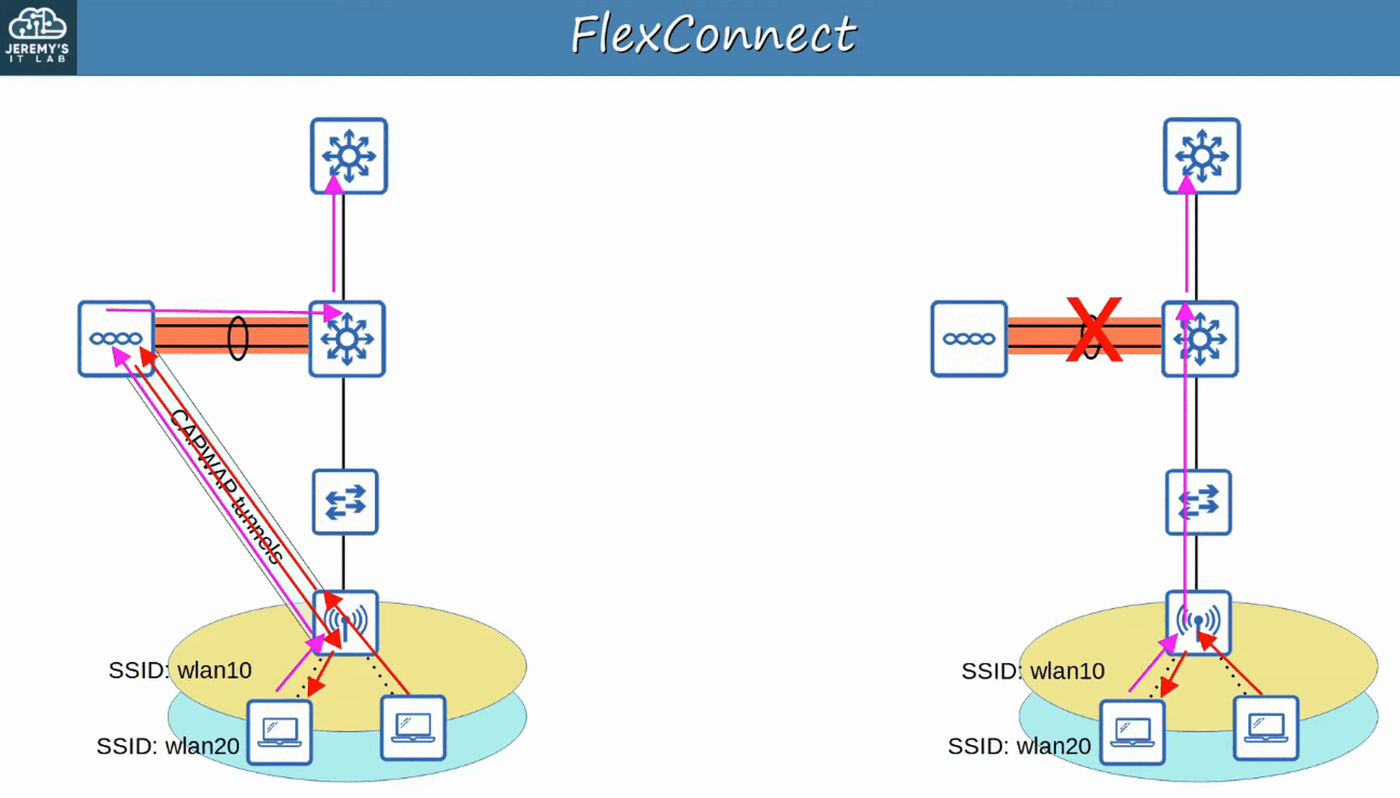
\includegraphics[keepaspectratio,alt={image}]{images/59-wireless-architecutres/img-006.png}}
\end{figure}

\begin{itemize}
\tightlist
\item
  SNIFFER

  \begin{itemize}
  \tightlist
  \item
    The AP does NOT OFFER a BSS for CLIENTS
  \item
    Dedicated to CAPTURING 802.11 FRAMES and SENDING them to a DEVICE
    running software such as WIRESHARK
  \end{itemize}
\item
  MONITOR

  \begin{itemize}
  \tightlist
  \item
    The AP does NOT OFFER a BSS for CLIENTS
  \item
    Dedicated to RECEIVING 802.11 FRAMES to detect ROGUE DEVICES
  \item
    If a CLIENT is found to be a ROGUE DEVICE, an AP can send
    DE-AUTHENTICATION MESSAGES to disassociate the ROGUE DEVICE from the
    AP
  \end{itemize}
\item
  ROGUE DETECTOR

  \begin{itemize}
  \tightlist
  \item
    The AP does not even USE its RADIO
  \item
    It LISTENS to traffic on the WIRED NETWORK only, but it receives a
    list of SUSPECTED ROGUE CLIENTS and AP MAC ADDRESSES from the WLC
  \item
    By LISTENING to ARP MESSAGES on the WIRED NETWORK and correlating it
    with the information it receives from the WLC, it can DETECT ROGUE
    DEVICES
  \end{itemize}
\item
  SE-CONNECT (SPECTRUM EXPERT CONNECT)

  \begin{itemize}
  \tightlist
  \item
    The AP does NOT OFFER a BSS for CLIENTS
  \item
    Dedicated to RF SPECTRUM ANALYSIS on ALL CHANNELS
  \item
    It can send information to software such as Cisco Spectrum Expert on
    a PC to COLLECT and ANALYZE the DATA
  \end{itemize}
\item
  BRIDGE / MESH

  \begin{itemize}
  \tightlist
  \item
    Like the AUTONOMOUS APs \emph{OUTDOOR BRIDGE} mode, the LIGHTWEIGHT
    AP can be a DEDICATED BRIDGE between SITES (Example: over LONG
    distances)
  \item
    A MESH can be made between the ACCESS POINTS
  \end{itemize}
\item
  FLEX PLUS BRIDGE

  \begin{itemize}
  \tightlist
  \item
    Adds FLEXCONNECT functionality to the BRIDGE / MESH mode
  \item
    Allows WIRELESS ACCESS POINTS to locally forward traffic even if
    connectivity to the WLC is lost
  \end{itemize}
\end{itemize}

\begin{figure}
\centering
\pandocbounded{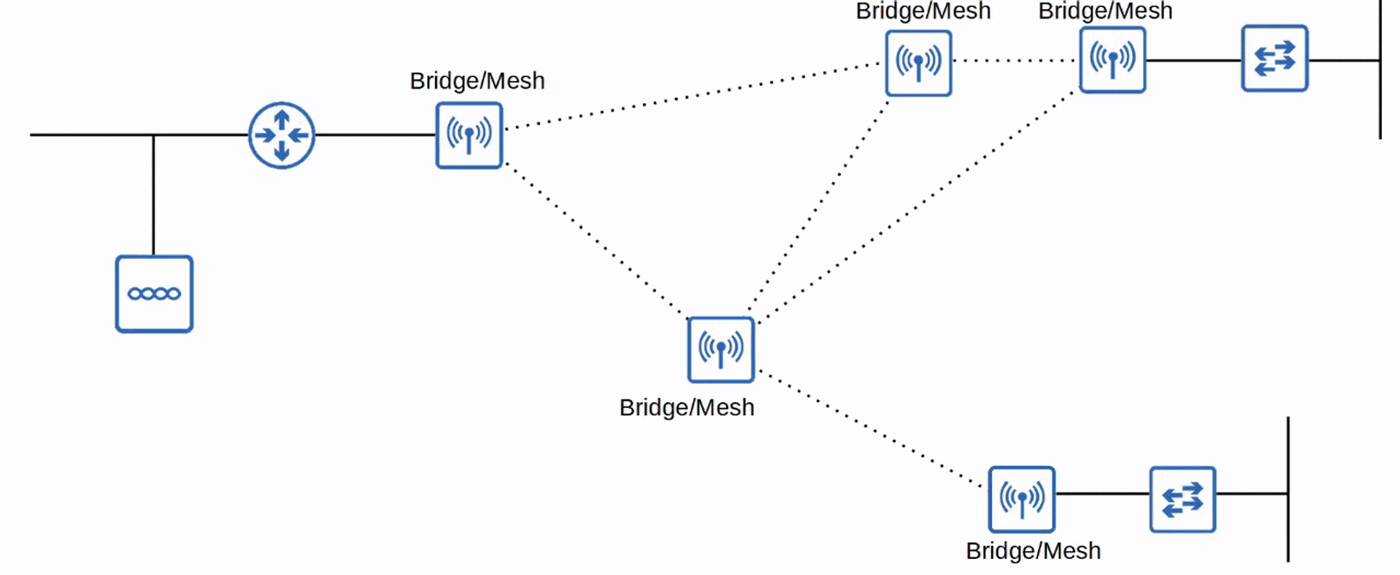
\includegraphics[keepaspectratio,alt={image}]{images/59-wireless-architecutres/img-007.png}}
\end{figure}

CLOUD-BASED APs

\begin{itemize}
\tightlist
\item
  CLOUD-BASED AP architecture is between AUTONOMOUS AP and SPLIT-MAC
  ARCHITECTURE

  \begin{itemize}
  \tightlist
  \item
    AUTONOMOUS APs that are centrally managed in the CLOUD
  \end{itemize}
\item
  CISCO MERAKI is a popular CLOUD-BASED WI-FI solution
\item
  The MERAKI dashboard can be used to configure APs, monitor the
  NETWORK, generate performance reports, etc.

  \begin{itemize}
  \tightlist
  \item
    MERAKI also tells each AP which CHANNEL to use, what transmit power,
    etc.
  \end{itemize}
\item
  However, DATA TRAFFIC is not sent to the CLOUD. It is sent directly to
  the WIRED NETWORK like when using AUTONOMOUS APs

  \begin{itemize}
  \tightlist
  \item
    Only management / control traffic is sent to the CLOUD
  \end{itemize}
\end{itemize}

\begin{figure}
\centering
\pandocbounded{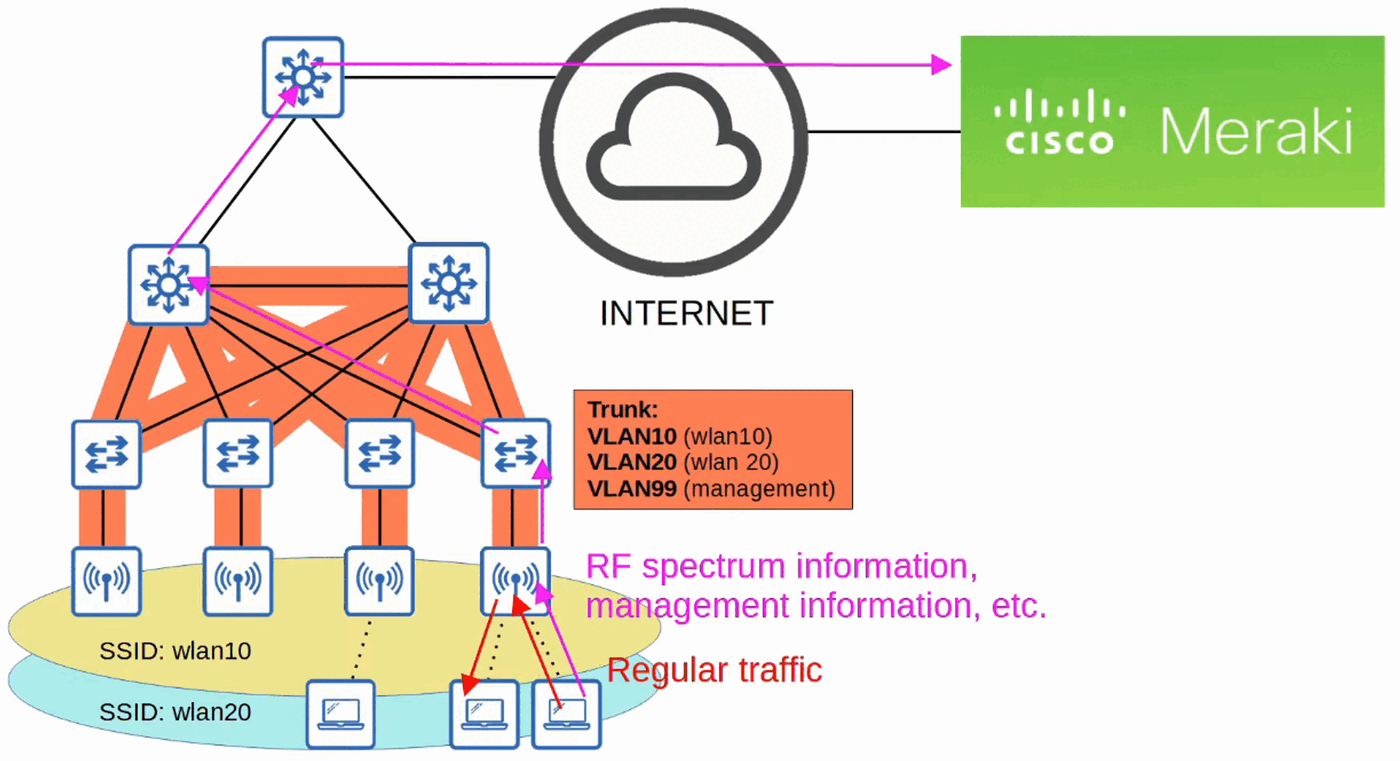
\includegraphics[keepaspectratio,alt={image}]{images/59-wireless-architecutres/img-008.png}}
\end{figure}

\begin{figure}
\centering
\pandocbounded{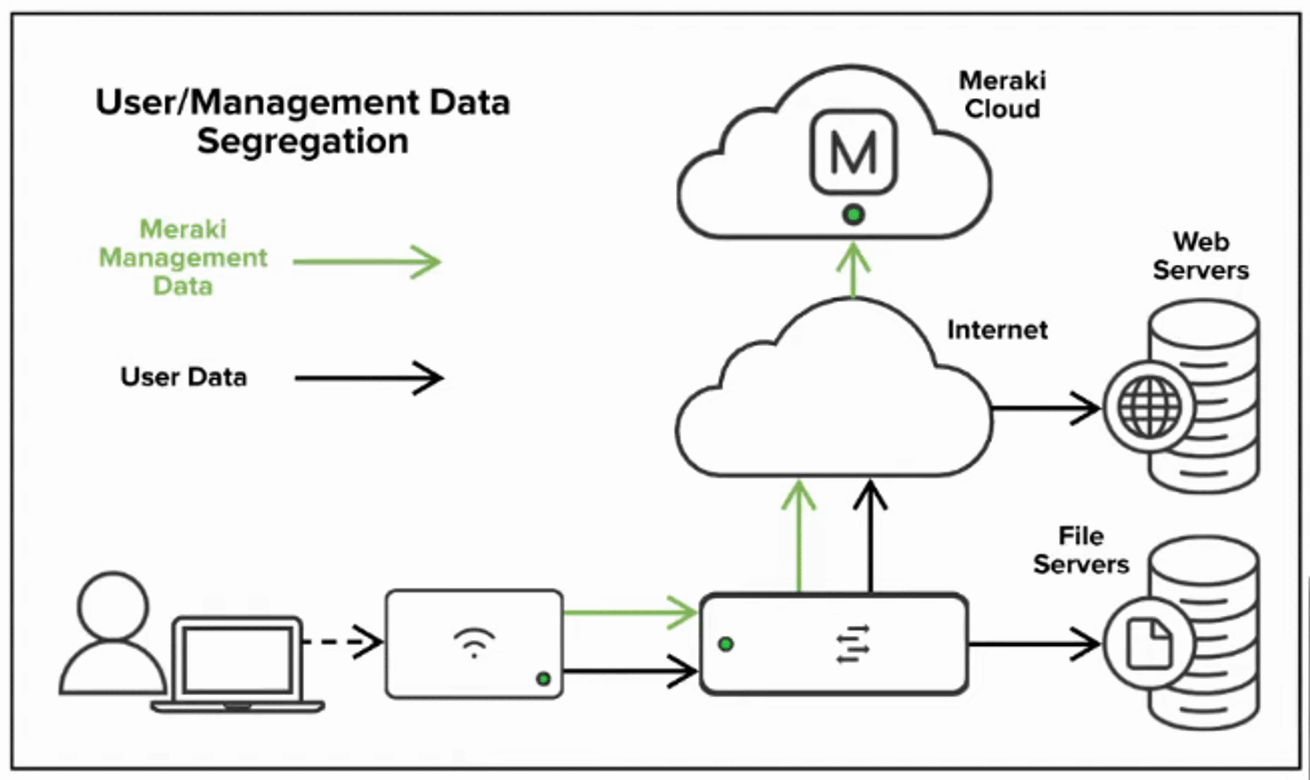
\includegraphics[keepaspectratio,alt={image}]{images/59-wireless-architecutres/img-009.png}}
\end{figure}

\section{Wireless LAN Controller (WLC)
Deployments}\label{wireless-lan-controller-wlc-deployments}

\begin{itemize}
\tightlist
\item
  In a SPLIT-MAC ARCHITECTURE, there FOUR MAIN WLC DEPLOYMENT MODES:

  \begin{itemize}
  \tightlist
  \item
    UNIFIED

    \begin{itemize}
    \tightlist
    \item
      THE WLC is a HARDWARE APPLICANCE in a central location of the
      NETWORK
    \end{itemize}
  \item
    CLOUD-BASED

    \begin{itemize}
    \tightlist
    \item
      The WLC is a VM running on a SERVER, usually in a PRIVATE CLOUD in
      a DATA CENTER
    \item
      This is NOT the same as the CLOUD-BASED AP ARCHITECTURE discussed
      previously
    \end{itemize}
  \item
    EMBEDDED

    \begin{itemize}
    \tightlist
    \item
      The WLC is integrated within a SWITCH
    \end{itemize}
  \item
    MOBILITY EXPRESS

    \begin{itemize}
    \tightlist
    \item
      THE WLC is integrated within an AP
    \end{itemize}
  \end{itemize}
\end{itemize}

\section{Unified WLC}\label{unified-wlc}

\begin{itemize}
\tightlist
\item
  THE WLC is a HARDWARE APPLICANCE in a central location of the NETWORK
\item
  A UNIFIED WLC can support up to about 6000 APs
\item
  If more than 6000 APs are needed, additional WLCs can be added to the
  NETWORK
\end{itemize}

\begin{figure}
\centering
\pandocbounded{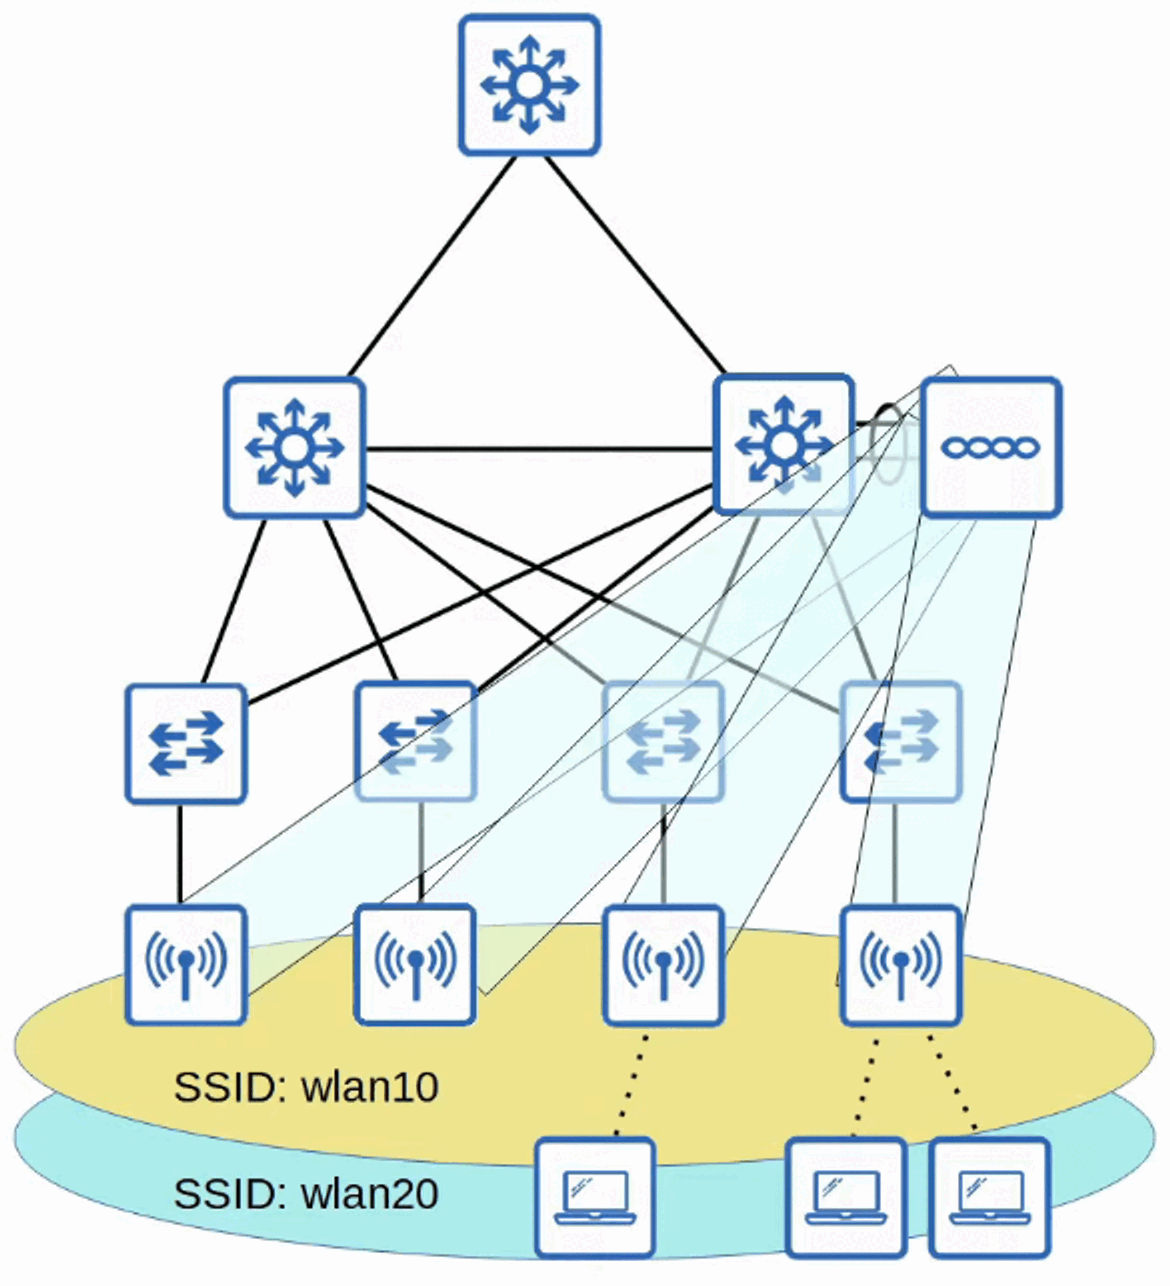
\includegraphics[keepaspectratio,alt={image}]{images/59-wireless-architecutres/img-010.png}}
\end{figure}

\section{Cloud-Based}\label{cloud-based}

\begin{itemize}
\tightlist
\item
  The WLC is a VM running on a SERVER, usually in a PRIVATE CLOUD in a
  DATA CENTER
\item
  CLOUD-BASED WLCs can typically support up to about 3000 APs
\item
  If more than 3000 APs are needed, more WLC VMs can be deployed
\end{itemize}

\begin{figure}
\centering
\pandocbounded{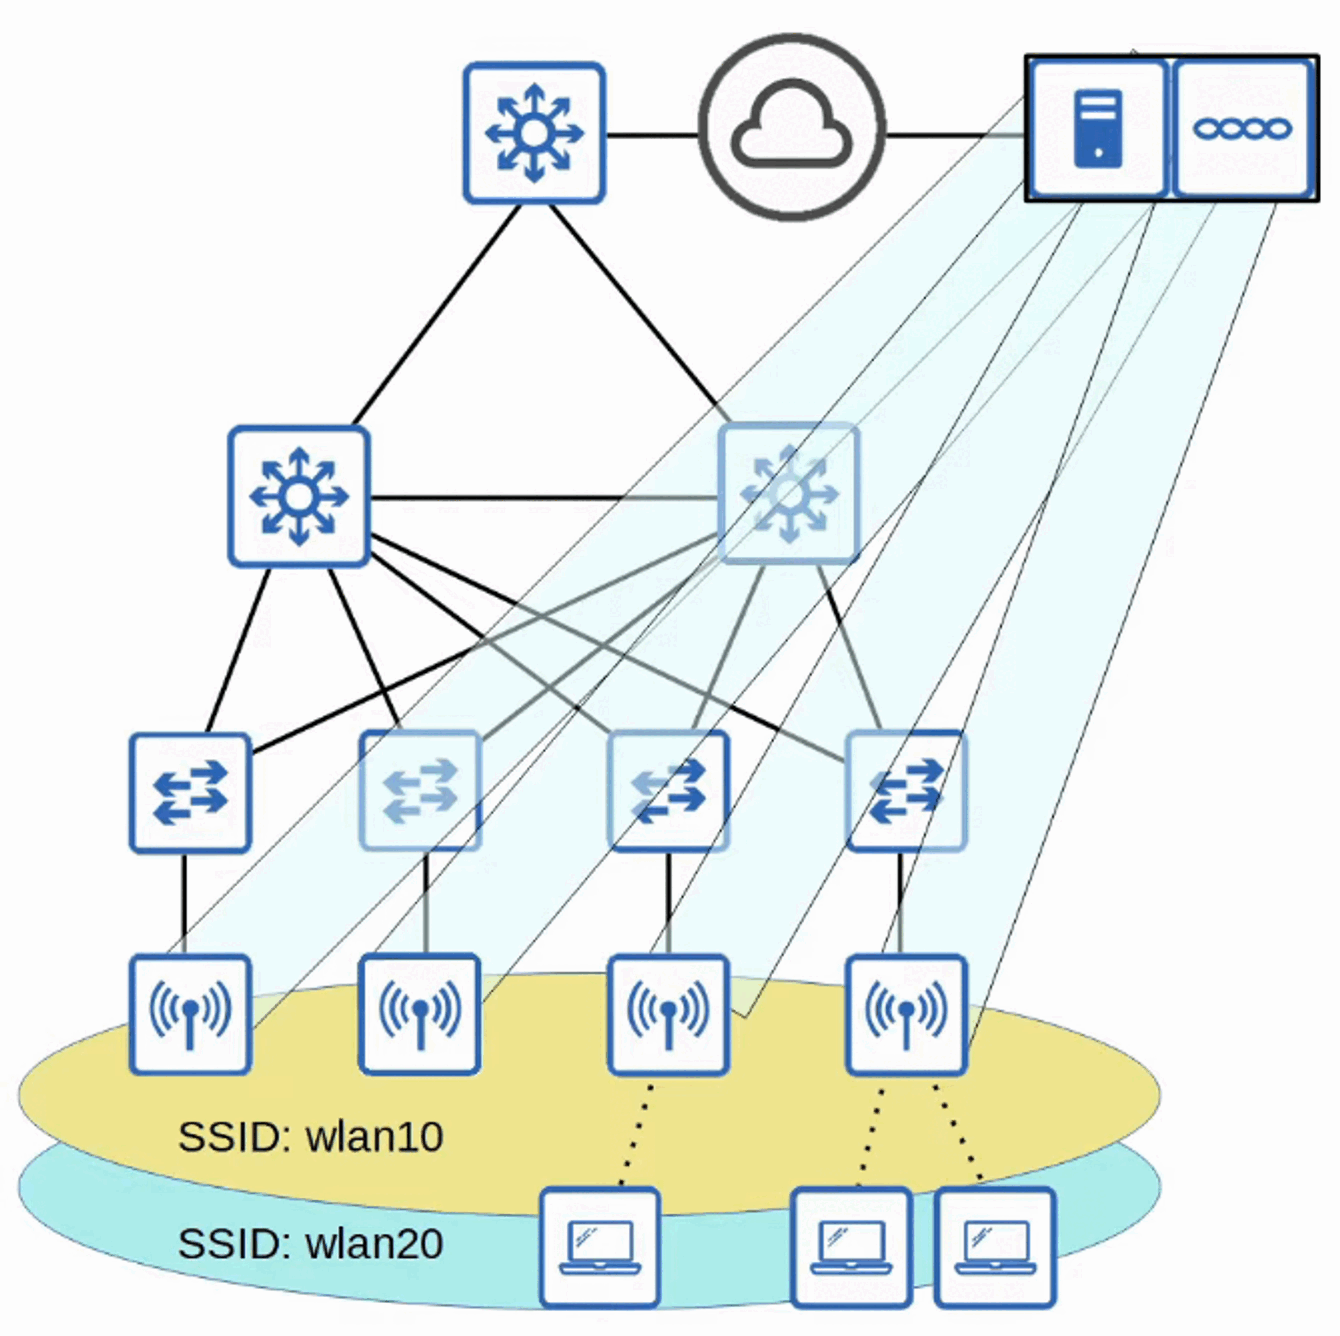
\includegraphics[keepaspectratio,alt={image}]{images/59-wireless-architecutres/img-011.png}}
\end{figure}

\section{Embedded WLC}\label{embedded-wlc}

\begin{itemize}
\tightlist
\item
  The WLC is embedded within a SWITCH
\item
  An EMBEDDED WLC can support up to about 200 APs
\item
  If more than 200 APs are needed, more SWITCHES with EMBEDDED WLCs can
  be added
\end{itemize}

\begin{figure}
\centering
\pandocbounded{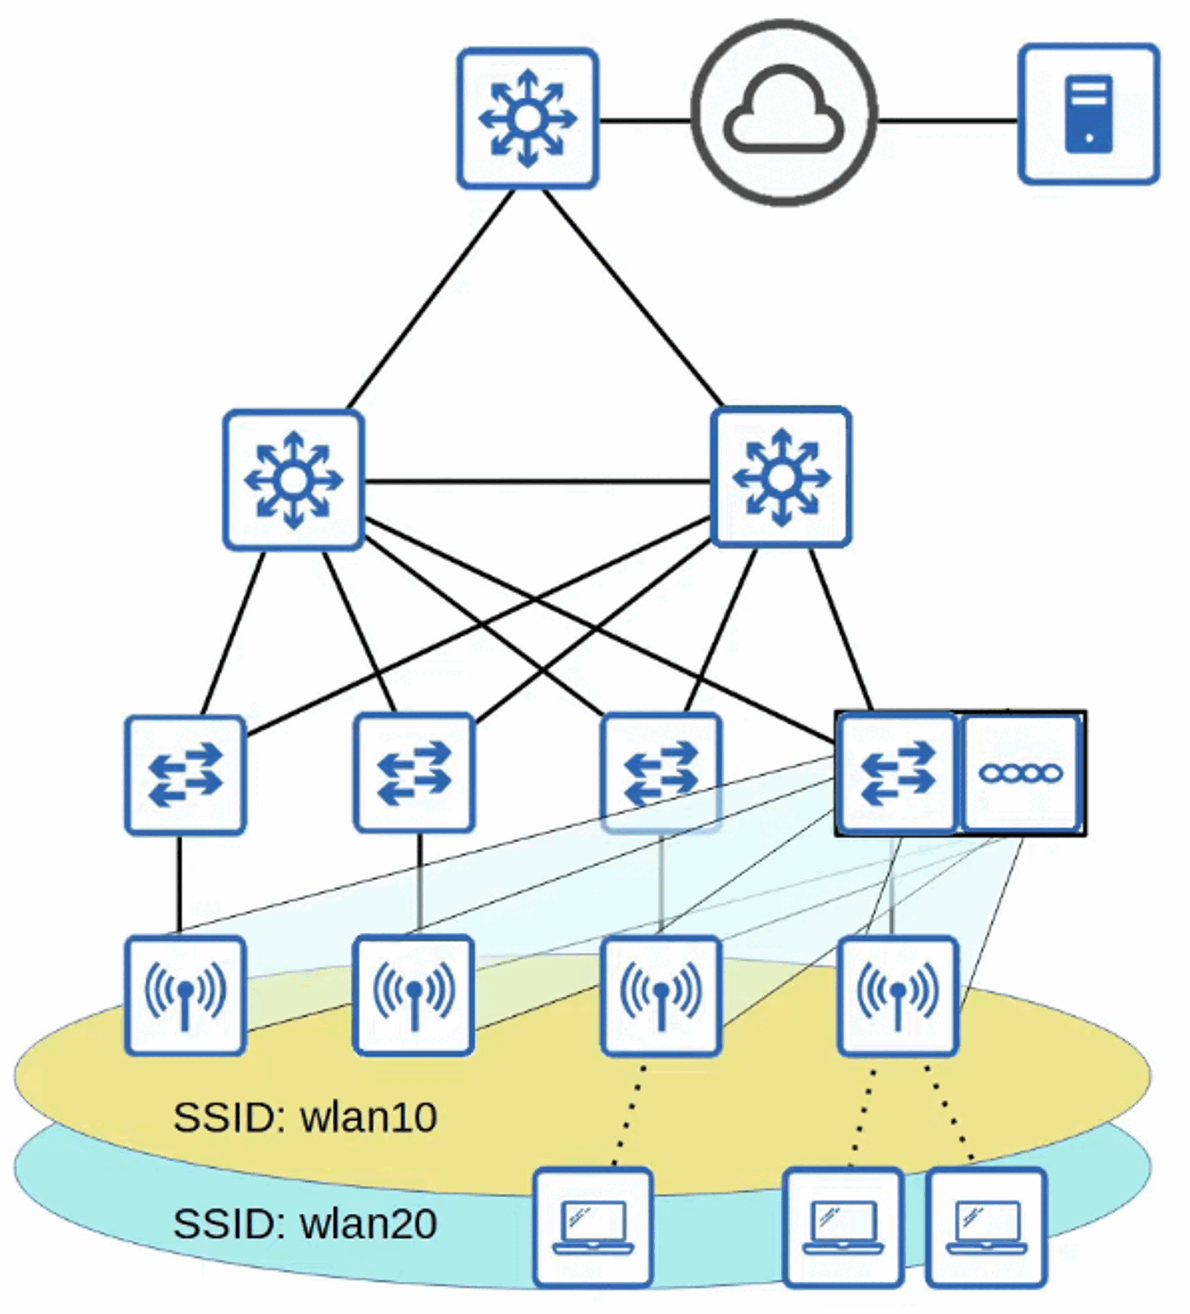
\includegraphics[keepaspectratio,alt={image}]{images/59-wireless-architecutres/img-012.png}}
\end{figure}

\section{Cisco Mobility Express WLC}\label{cisco-mobility-express-wlc}

\begin{itemize}
\tightlist
\item
  The WLC is embedded within an AP
\item
  A MOBILITY EXPRESS WLC can support up to about 100 APs
\item
  If more than 100 APs are needed, more APs with EMBEDDED MOBILITY
  EXPRESS WLCs can be added
\end{itemize}

\begin{figure}
\centering
\pandocbounded{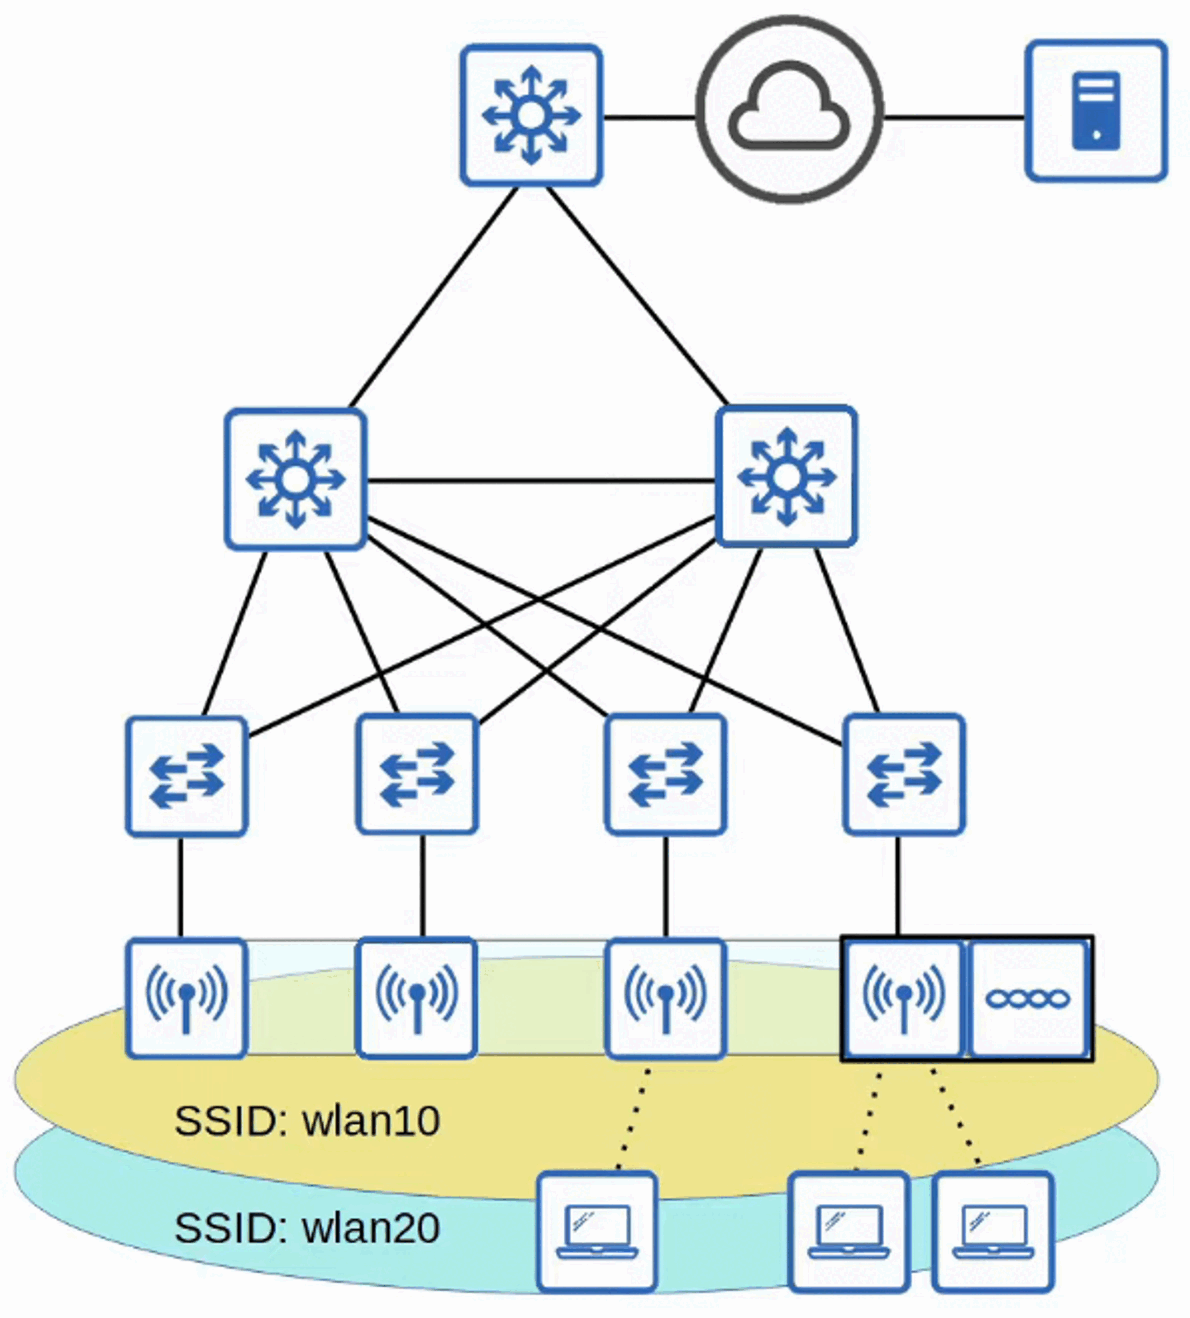
\includegraphics[keepaspectratio,alt={image}]{images/59-wireless-architecutres/img-013.png}}
\end{figure}
